\documentclass[/Users/ikedahajime/GitHub/reserch/master_report/thesis]{subfiles}

% このファイル内だけのコマンド
\begin{document}
\chapter{序論}

% \section{研究背景}
自らの力で進むものは世の中に多く存在する。魚や鳥、人などをはじめとした生物はその典型的な例である。
%図を挿入;
\begin{figure}
    \centering
    \begin{tabular}{c}%TODO:バランス
        \begin{minipage}{0.3\hsize}
            \text{(a)}
            \includegraphics[width=\textwidth]{img/intro/256px-School_of_sardines_at_the_Monterey_Bay_Aquarium_(12056).jpg}
        \end{minipage}
        \begin{minipage}{0.3\hsize}
            \text{(b)}
            \includegraphics[width=\textwidth]{img/intro/mukudori.png}
        \end{minipage}\\
        \begin{minipage}{0.3\hsize}
            \text{(c)}
            \includegraphics[width=\textwidth]{img/intro/thumbnail.png}
        \end{minipage}
        \begin{minipage}{0.25\hsize}
            \text{(d)}
            \includegraphics[width=\textwidth]{img/intro/ants_volt.pdf}
        \end{minipage}
    \end{tabular}
    \caption[Four sample images]
    {
        アクティブマターの例。 (a) イワシのトルネード\cite{school_of_fish} (b) 椋鳥の群れ\cite{mukudori_group} (c)枯草菌\cite{dombrowskiSelfConcentrationLargeScaleCoherence2004}
        (d)蟻の群れ\cite{schneirla1944unique}
    }
    \label{fig:example_actmat}
\end{figure}
これらの生物は、単独では一見無秩序な運動を行う。しかし多くの個体が集まって集団になると、\figref{fig:example_actmat}
のようにイワシのトルネード、
椋鳥の群れなどのように、群れ全体が秩序だった集団運動を行う。この集団運動は特定の個体がリーダーとなって
指示を出すことで起こっているのではなく、各個体同士の相互作用の結果として発生している。
このような自らの力で進むものやその集団のことを総称してアクティブマターと呼ぶ。アクティブマターは
環境からエネルギーを取り出し、それ自身が前を進みエネルギーを生成する。このような特徴から
アクティブマターは非平衡な物質であるため、非平衡統計力学の観点から近年注目を集めている。%TODO繋ぎ;b

アクティブマターの特徴の1つとして、自発的な渦の発生があげられる。
この現象は個々の構成要素が自己駆動することによって起こる現象であり、
このような系では、\figref{fig:intro_flow}のように速度相関が発達する。相関長はある特徴的な長さを持っており、
この長さは渦の大きさに関係していることがわかっている。
この現象は様々なアクティブマター系において観測されている。
例えば枯草菌\cite{wensinkMesoscaleTurbulenceLiving2012}や大腸菌\cite{pengImagingEmergenceBacterial2021}
など多くの系で見ることができ、理論においてもToner-Tu-SwiftHohenberg (TTSH) 方程式など\cite{wensinkMesoscaleTurbulenceLiving2012}様々な系で見られる。%:toner-toとか
% 円領域に行った方が自然?円形領域に閉じ込めるとまわる〜
\begin{figure}%TODO:増やす
    \centering
    \begin{tabular}{c}
        \begin{minipage}{0.6\hsize}
            % \text{(a)}
            \includegraphics[width=\textwidth]{img/intro/abd1240-f1.jpeg}
        \end{minipage}

    \end{tabular}
    \caption[Four sample images]
    {
        障害物の影響がない系における大腸菌の渦度\cite{pengImagingEmergenceBacterial2021}
    }
    \label{fig:intro_flow}
\end{figure}
\begin{figure}
    \centering
    \begin{tabular}{c}
        \begin{minipage}{0.6\hsize}
            % \text{(a)}
            \includegraphics[width=\textwidth]{img/intro/circle_ecoil.pdf}
        \end{minipage}
    \end{tabular}
    \caption[Four sample images]
    {
        円の中に閉じ込められた大腸菌が形成する渦\cite{beppuGeometrydrivenCollectiveOrdering2017}
    }
    \label{fig:intro_confine}
\end{figure}


これらアクティブマターについての理論研究はその多くが境界のないバルク系であるが、
閉じ込め系に対する研究も行われている。閉じ込め系においてはその境界の形状などによって%解説?
様々な現象が見られている。例えば粒子の凝集\cite{dasAggregateMorphologyActive2020}、整流効果\cite{ghoshSelfPropelledJanusParticles2013}
捕集効果\cite{kaiserHowCaptureActive2012}、エッジ流\cite{soniOddFreeSurface2019}などが観測されている。
そのような現象の1つとして、\figref{fig:intro_confine}のようにアクティブマターを円形領域の中に入れると、その
円の半径によって円の中に1つ、あるいは複数の渦が発生することが知られている。
この渦は、円の半径と系が持つ相関長が等しくなる時、
\figref{fig:intro_confine}のように1つになることが分かっている。
この現象は、この障害物とアクティブマターとの相互作用によって相関長
を取り出すことができると言える。この現象は実験、理論ともに研究が進んでいる。
特に理論研究においては、円の中に閉じ込めた時に渦一つが現れるだけでなく、
複数の渦が現れる、群れが振動するなど、様々な現象が見られている。
しかしこれらの理論研究においては、方程式に整列相互作用や流体力学相互作用を顕に入れる、
あるいは粒子の形状を変化させてその向きを揃える効果を入れるなど、複雑な条件を持った
モデルが主に使われている。これらの効果は現実のアクティブマターの動きをよく再現する一方で、
これらの効果は複雑であり、これらのない、自己駆動力のみによる効果も研究されている。
%TODO:図の追加:シミュレーションのconfine

そのようなシンプルな状態を研究するためのモデルとして代表的なモデルが Active Brownian Particles (ABP) モデルである。
ABPモデルは以下のように表される。
\begin{eqnarray}\label{eq:eom_abp_1}
    \dot{\bm{r}_i}(t)&=& \frac{1}{\zeta}\bm{F}_i + v_0 \bm{e}(\theta_i(t))
\end{eqnarray}
\begin{eqnarray}\label{eq:eom_abp_2}
    \dot{\theta_i }(t) &=& \sqrt{\frac{2}{\tau_p}}\eta_i(t)
\end{eqnarray}
ここで、\mbox{\boldmath$r$}は粒子の位置、$v_0$ は自己推進の速度、$\zeta$ は摩擦係数を表す。
$\eta_i$ はホワイトノイズで、$\langle \eta_i(t) \eta_j(t') \rangle=\delta_{ij}\delta(t-t')$の関係を満たす。
ここで、$\langle \dots \rangle$ はアンサンブル平均である。
$\mbox{\boldmath$e$}(\theta_i)=(\cos\theta_i,\sin \theta_i)$は自己推進の方向を表す単位ベクトルで、
$\tau_p$は持続時間である。
\begin{figure}
    \centering
    \begin{tabular}{c}
        \begin{minipage}{0.7\hsize}
            % \text{(a)}
            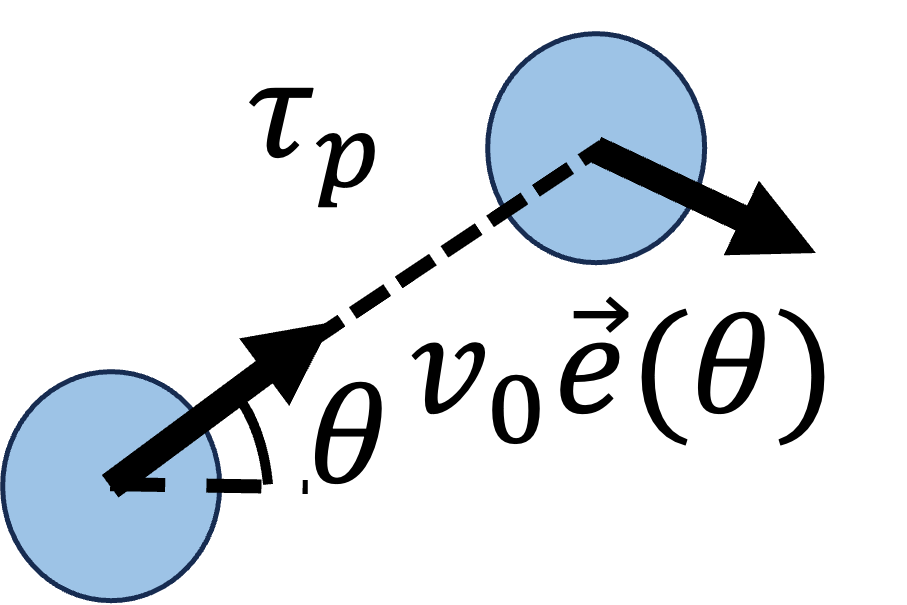
\includegraphics[width=\textwidth]{img/intro/fig_abp_model.png}
        \end{minipage}
    \end{tabular}
    \caption[Four sample images]
    {
        ABPモデルの模式図
    }
    \label{fig:intro_saple_abp}
\end{figure}
\equref{eq:eom_abp_1}は平衡系におけるブラウン運動に似た形を持つ。唯一の違いは違いは右辺第2項であり、
この項は角度$\theta_i$の方向に、速度$v_0$で進むことを表す。
その角度$\theta_i$の拡散には持続時間$\tau_p$が程度の時間がかかる。つまりこの粒子は、
\figref{fig:intro_saple_abp}のように
典型的には速度$v_0$でその進行方向を時間$\tau_p$の間変えず同じ方向へ進み続ける。


このモデルは整列相互作用や流体力学相互作用などの複雑な相互作用が顕に
入っていないシンプルなモデルである。%TODO:その性質からあと2、3行
そのシンプルさにも関わらず、
様々な非平衡現象が観測されている。%列強:MIPS,うずetc->障害物
ABP モデルにおける典型的な研究対象の一つは Motility-Induced Phase Separation(MIPS) である。
これは自発的に粒子が密集して密度が高い部分と低い部分に分かれる現象である。
これは粒子間の引力相互作用がない場合でも起きる現象であり、平衡系の粒子間引力による相分離と対照的である。
また、この粒子集団において速度相関が発達することが分かっている。


近年、この渦度の発達は MIPS が発生しない系においても起こることが分かった。
これらの研究では、 MIPS の発生を防ぐために高密度領域を探索する\cite{szamelLongrangedVelocityCorrelations2021}、
ABPモデルに慣性の効果を加えた inertial inertial Active Brownian Particles(iABP) モデルを用いる\cite{kurodaAnomalousFluctuationsHomogeneous2023}、
粒子の進行方向の回転対称性を破った Chiral Active Brownian Particlesモデル\cite{kurodaLongrangeTranslationalOrder2024}
において観測されている。

ABP 系においては、障害物との相互作用についても研究されている。
この系においても、実験と同様に粒子の凝集や整流効果などの現象が観測されている。
円形領域への閉じ込めと速度相関の関係についても議論されている\cite{capriniCollectiveEffectsConfined2021}。
しかし、この論文において粒子を閉じ込めている壁は1粒子分の幅を持つリング状の壁である。
つまりこの系は1次元系であり、実験系と比べると極端な状態であると言える。
そこで本研究では、閉じ込めの条件を2次元の円形領域に拡張してシミュレーションを行なった。
具体的には、 ABP を2次元の円形領域に閉じ込め、様々なパラメータを変化させてその
ダイナミクスを観測した。


さらに、相関長と閉じ込めによる効果の関係をより明らかにするため、CABP を用いた。
CABPにおいてもバルク系における速度相関の発達については見られている\cite{kurodaLongrangeTranslationalOrder2024}。
このモデルでは Caprini らによって、引力相互作用を用いて粒子を1つの塊にして、その塊の挙動を見る研究が行われている\cite{capriniSelfrevertingVorticesChiral2024}が、
この研究では塊全体が一方向に回る状態と振動する状態の遷移については議論されているが、
相関長との関係については議論されていない。
そこで本研究ではこの粒子をを円形領域に閉じ込め、粒子の回転半径 $R_\Omega$ を変化させて
同様に流れや渦について調べた。


また、実験系においてはアクティブマターを閉じ込める壁の形状による効果も研究されている。%TODO:ずを挿入
その中にはアクティブマターによる渦同士の相互作用について研究しているものがある。
Wioland らは枯草菌を複数の円が格子状に配置された領域に閉じ込めてその渦について調べた\cite{wiolandFerromagneticAntiferromagneticOrder2016}。
これらの円は細い流路によって繋がっており、それを通じて隣り合った渦が相互作用する。
この研究においては、それぞれの円における渦の向きを電子系におけるスピンに例え、
それらの渦が強磁性的、つまり渦が同じ方向に向かって回るのか、あるいは反強磁性的、
つまり隣り合う渦同士が反対の方向に向かって回るのかについて調べた。
その結果、流路の幅が大きく相互作用が強いと強磁性的秩序を示し、
逆に流路の幅が小さくなって相互作用が弱まると反強磁性的秩序を示した。
さらに、前田らによってこの渦秩序が幾何学的に解釈されることが分かった\cite{beppuGeometrydrivenCollectiveOrdering2017}。
この研究では、二つの円を直接繋げて、それらの円における渦が強磁性的か反強磁性的かを調べた。
結果、渦の大きさによらず二つの円の距離のみによって強磁性状態と反強磁性状態が遷移することが分かった。
本研究では、この研究における自己駆動力の果たす役割について調べるため、 ABP を用いて解析を行なった。


% \section{本研究の目的と方法}
% \section{本論文の構成}
本論文は以下の構成からなる。
第1章では本論文の位置づけおよび、本論文の構成について述べる。
% 第2章では本研究に関連する先行研究について説明を行う.
第2章では数値計算手法および、その設定について説明を行う。
第3,4章では本研究で得た主要な結果について述べる。
第5章では本研究の結論と今後の展望に関して述べる。
付録Aでは本研究の形状による効果について述べた。
% 付録Bでは解析手法について詳細な説明を行う。
\end{document}
